\lhead{Date: 26/07/2021}  % For date in header

% REMOVE the % sign in the above lines if you want to
% compile this experiment file separately.

\begin{document}
	
	\chapter{Study of p-n Junction} % Replace the text with the title of the experiment
	\vspace{-1cm}
	\dateofexp{Date of Experiment: 26/07/2021} 
	% To display date in contents page
	
	\begin{center}% To display date of experiment in the title
		Date of Experiment: 26/07/2021
	\end{center}
	
	%%%%%%%%%%%%%%%%%%%%%%%%%%%%%%%%%%%%%%%%%%%%%
	% THE EXPERIMENT STARTS HERE %
	%%%%%%%%%%%%%%%%%%%%%%%%%%%%%%%%%%%%%%%%%%%%%
	
	\section{Aim}
	\begin{itemize}
%		\item 	To study the material characteristics of a p-n junction diode.
		\item 	To observe the dependence of depletion layer capacitance on reverse voltage
	\end{itemize}
	
	\section{Requirements}
	\begin{itemize}
		\item 	PN-Junction setup Model PN-1
		\item 	Sample: BC 109C (Base Emitter Junction)
		\item 	Cathode Ray Oscilloscope
	\end{itemize}
	
	\section{Theory}
%	The diode current equation for a forward biased diode is
%	given as:
%	\begin{equation}{\label{eqn:diode-eqn}}
%		I = I_s \left( \exp \dfrac{qV}{\eta kT} - 1 \right)
%	\end{equation}
	In the this of the experiment we will be studying the variation of depletion layer capacitance with reverse bias voltage. The depletion layer between the n- and p-sides of a pn junction diode serves as an insulating region that separates the two diode contacts. Thus, the diode in reverse bias exhibits a depletion-layer capacitance, sometimes more vaguely called a junction capacitance, analogous to a parallel plate capacitor with a dielectric between the contacts. In reverse bias the width of the depletion layer is widened with increasing reverse bias V , and the capacitance is accordingly decreased. Thus, the junction serves as a voltage-controllable capacitor. In a simplified one-dimensional model, the junction capacitance is
	\begin{equation}{\label{eqn:Cd}}
		C_d = K\epsilon_0 \dfrac{A}{\omega(V)}
	\end{equation}
	where $ A $ is the area, $ \omega (V) $ is the width of the depletion layer which is a function of reverse bias voltage, $ V $, $ K $ is the dielectric constant and $ \epsilon_0 $ is the permittivity of free space. 
	
	We will observe the variation of depletion layer capacitance with reverse bias voltage. From the above relation \ref{eqn:Cd} we can see that $ C_d $ is inversely proportional to $ V $. To do this we use the circuit shown below: an op-amp in inverting mode with $ V_{\mathrm{in}} $ being the input voltage, and the diode in place of $ R_{\mathrm{in}} $. If the diode has capacitance $ C_d $ then the reactance, $ \chi_C $ is given as $ 1/(j\omega C_d) $. Also, the gain of op-amp in inverting mode is given as $ V_{\mathrm{out}}/V_{\mathrm{in}} = -R_f/R_i$. So, the output voltage $ V_1 $ for an input signal of voltage $ V $ and frequency, $ \omega_1 $ is given by
	\begin{equation}{\label{eqn:V1}}
		V_1 = -\dfrac{R}{\chi_C}V = -Rj \omega_1 C_d V
	\end{equation}
	Similarly, the output voltage $ V_2 $ for an input signal of voltage $ V $ and frequency, $ \omega_2 $ is given as:
	\begin{equation}{\label{eqn:V2}}
		V_2 = -\dfrac{R}{\chi_C}V = -Rj \omega_2 C_d V
	\end{equation}
	From the above equations, we obtain
	\begin{equation}{\label{eqn:Cd-final}}
		C_d = \dfrac{1}{VR}\dfrac{\sqrt{V_2^2 - V_1^2}}{\sqrt{\omega_2^2 - \omega_1^2}} = 0.41\sqrt{V_2^2 - V_1^2} \ \text{\si{\pico\farad}}
	\end{equation}
	for the values $ V = \SI{200}{\milli\volt} $, $ R = \SI{100}{\kilo\ohm} $, $ \omega_1 = 2 \pi 5\,\si{\kilo\hertz} $ and $ \omega_1 = 2 \pi 20\,\si{\kilo\hertz} $ used in the apparatus.
	\begin{figure}
		\centering
		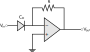
\includegraphics{Experiments/sem12-pn-circuit.pdf}
	\end{figure}
	
\section{Procedure}

\begin{enumerate}
	\item 	Connect the CRO to the setup.
	\item 	For this experiment the diode is to be connected to the left socket of the setup.
	\item 	Set the display 2 to \texttt{BIAS} mode.
	\item 	Measure and note down the peak to peak output voltage in the CRO for different bias voltages and frequencies.
	\item  	Calculate $ C_d $ and plot a graph of $ C_d $ versus Junction voltage, $ V $.
	
\end{enumerate}

\section{Observation and graph}

\begin{table}[h]
\centering
\begin{tabular}{|r|r|r|r|}
\hline
\rowcolor[HTML]{EFEFEF} 
\multicolumn{1}{|c|}{\cellcolor[HTML]{EFEFEF}\begin{tabular}[c]{@{}c@{}}Bias Voltage\\ (\si{\volt})\end{tabular}} & \multicolumn{1}{c|}{\cellcolor[HTML]{EFEFEF}\begin{tabular}[c]{@{}c@{}}$V_1$ \\ (\si{\milli\volt})\end{tabular}} & \multicolumn{1}{c|}{\cellcolor[HTML]{EFEFEF}\begin{tabular}[c]{@{}c@{}}$V_2$  \\ (\si{\milli\volt})\end{tabular}} & \multicolumn{1}{c|}{\cellcolor[HTML]{EFEFEF}\begin{tabular}[c]{@{}c@{}}$C_d$ \\ (\si{\pico\farad})\end{tabular}} \\ \hline
0.0                                                                                                      & 0                                                                                               & 0                                                                                                & 0.00                                                                                            \\ \hline
0.5                                                                                                      & 420                                                                                             & 500                                                                                              & 111.23                                                                                          \\ \hline
1.0                                                                                                      & 1080                                                                                            & 1300                                                                                             & 296.68                                                                                          \\ \hline
2.0                                                                                                      & 2500                                                                                            & 2200                                                                                             & 486.85                                                                                          \\ \hline
3.0                                                                                                      & 3800                                                                                            & 3000                                                                                             & 956.28                                                                                          \\ \hline
4.0                                                                                                      & 4800                                                                                            & 3200                                                                                             & 1,466.86                                                                                        \\ \hline
5.0                                                                                                      & 6400                                                                                            & 3200                                                                                             & 2,272.45                                                                                        \\ \hline
6.0                                                                                                      & 6400                                                                                            & 3600                                                                                             & 2,169.52                                                                                        \\ \hline
7.0                                                                                                      & 6200                                                                                            & 3600                                                                                             & 2,069.59                                                                                        \\ \hline
8.0                                                                                                      & 6000                                                                                            & 3600                                                                                             & 1,968.00                                                                                        \\ \hline
9.0                                                                                                      & 5400                                                                                            & 3400                                                                                             & 1,720.05                                                                                        \\ \hline
10.0                                                                                                     & 4200                                                                                            & 2600                                                                                             & 1,352.38                                                                                        \\ \hline
11.0                                                                                                     & 2500                                                                                            & 1600                                                                                             & 787.58                                                                                          \\ \hline
\end{tabular}
\caption{}
\label{tab:pn}
\end{table}
%
%
\begin{figure}[H]
	\centering
	\begin{tikzpicture}
		\begin{axis}[
			xlabel={Bias Voltage (\si{\volt})}, 
			ylabel={$ C_D $ (\si{\pico\farad})},
			grid=both,
			minor grid style={gray!25},
			major grid style={gray!25},
			width=0.75\linewidth,mark=*]
			\addplot[line width=1pt,color=blue,mark=*] %
			table[x=V,y=Cd,col sep=comma]{1208-data.csv};
		\end{axis}
	\end{tikzpicture}
	\caption{Plot of $ C_D $ versus bias voltage}
	\label{fig:1208-plot}
\end{figure}

\section{Result}
    The dependence of depletion layer capacitance on reverse bias voltage was observed and plotted.

\end{document}
